\documentclass{article}
\usepackage{a0size}
\renewcommand{\tiny}{\fontsize{12}{14}\selectfont}
\renewcommand{\scriptsize}{\fontsize{14.4}{18}\selectfont}   
\renewcommand{\footnotesize}{\fontsize{17.28}{22}\selectfont}
\renewcommand{\small}{\fontsize{20.74}{25}\selectfont}
\renewcommand{\normalsize}{\fontsize{24.88}{30}\selectfont}
\renewcommand{\large}{\fontsize{29.86}{37}\selectfont}
\renewcommand{\Large}{\fontsize{35.83}{45}\selectfont}
\renewcommand{\LARGE}{\fontsize{43}{54}\selectfont}
\renewcommand{\huge}{\fontsize{51.6}{64}\selectfont}
\renewcommand{\Huge}{\fontsize{61.92}{77}\selectfont}
\newcommand{\veryHuge}{\fontsize{74.3}{93}\selectfont}
\newcommand{\VeryHuge}{\fontsize{89.16}{112}\selectfont}
\newcommand{\VERYHuge}{\fontsize{107}{134}\selectfont}


\newcommand{\membersize}{\noindent\fontsize{61.92}{77}\selectfont}
\newcommand{\titlesize}{\noindent\fontsize{72}{80}\selectfont}

% These colours are tried and tested for titles and headers. Don't
% over use color!
\usepackage{color}

\definecolor{college-engineering}{rgb}{0.09,0.25,0.41}
\definecolor{dept-cse}{rgb}{0.26,0.58,0.82}

\renewcommand{\labelitemi}{\textcolor{college-engineering}\textbullet}
\renewcommand{\labelitemii}{\textcolor{college-engineering}{--}}

\setlength{\labelsep}{0.5em}


% see documentation for a0poster class for the size options here
\let\Textsize\normalsize
\def\Head#1{\hrule\smallskip\noindent{\huge\color{college-engineering} \textbf{#1}}\bigskip}
\def\Subhead#1{\noindent{\large\color{college-engineering} #1}\bigskip}


\usepackage{pgfplots}
\usepackage{lipsum}  

\usepackage[
  paperwidth=90cm,
  paperheight=120cm,
  top=25cm,
  left=9cm,
  right=9cm,
]{geometry}


\usepackage{wallpaper}
\CenterWallPaper{1}{assets/background}

\usepackage{fontspec}
\setmainfont{Arial}

\usepackage[BoldFont, SlantFont]{xeCJK}
\setCJKmainfont{Microsoft JhengHei}

\usepackage[absolute]{textpos}
\TPGrid[80mm,390mm]{15}{12}

\parindent=0pt
\parskip=\baselineskip

\begin{document}
% disable page numbering
\thispagestyle{empty}
\membersize \textbf{第17組:朱劭璿、陳居廷}\hspace{20.5cm}\textbf{指導老師:陳嘉平 教授}
\bigskip

\titlesize \textbf{TSM-Net: 以對抗式時序壓縮自編碼器為基礎的音訊變速演算法 \\
TSM-Net: Temporal Compressing Autoencoder with Adversarial Losses for Time-Scale Modification on Audio Signals}

\begin{textblock}{7.0}(0,0)
\Head{Introduction} \\
\Large \lipsum[1-1] \\

\medskip
\Head{Related Works} \\
\Large \lipsum[2-2] \\

\medskip
\Head{Methodology} \\
\Large \lipsum[3-3]
\end{textblock}

\begin{textblock}{7.0}(8,0)
\Head{Experiment} \\
\Large \lipsum[4-4]
\large \begin{figure}
\begin{center}
\begin{tabular}{l}
(a)
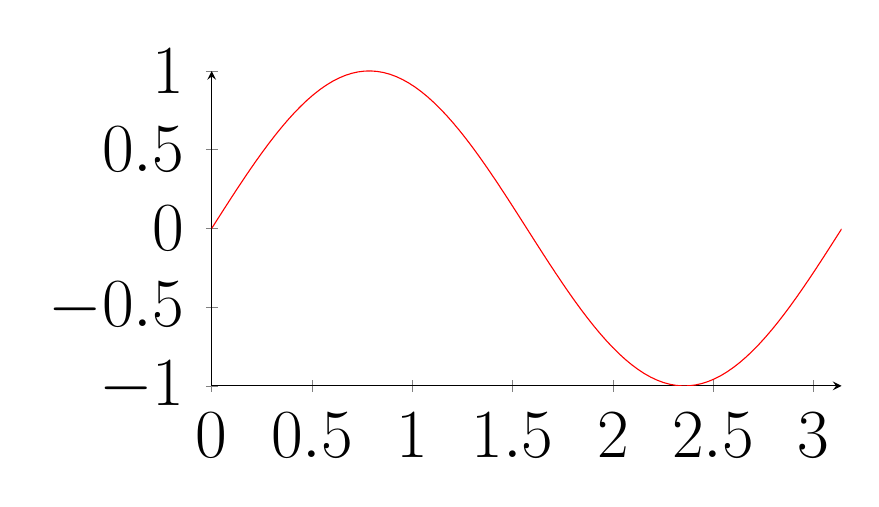
\begin{tikzpicture}
\begin{axis}[
  domain=0:3.14,
  axis lines = left,
  legend pos=outer north east,
  width=8cm,
  height=4cm,
  scale only axis,
]
\addplot [
  samples=100, 
  color=red,
]
{sin(deg(2*x))};

\end{axis}
\end{tikzpicture}

(b)
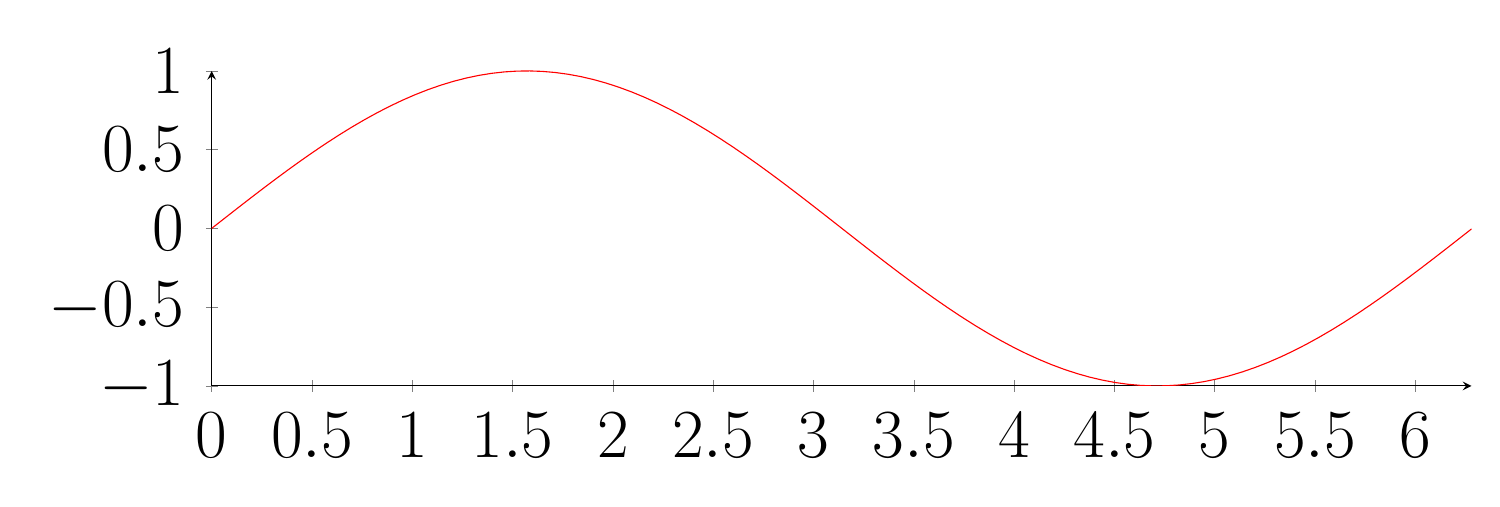
\begin{tikzpicture}
\begin{axis}[
  domain=0:6.28,
  axis lines = left,
  legend pos=outer north east,
  width=16cm,
  height=4cm,
  scale only axis,
]
\addplot [
  samples=100, 
  color=red,
]
{sin(deg(x))};

\end{axis}
\end{tikzpicture} \\

(c)
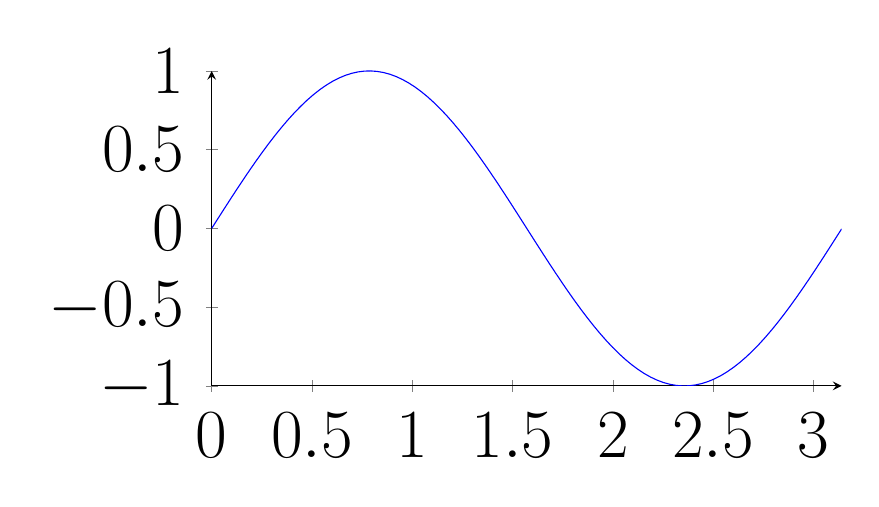
\begin{tikzpicture}
\begin{axis}[
  domain=0:3.14,
  axis lines = left,
  legend pos=outer north east,
  width=8cm,
  height=4cm,
  scale only axis,
]
\addplot [
  samples=100, 
  color=blue,
]
{sin(deg(2*x))};

\end{axis}
\end{tikzpicture}

(d)
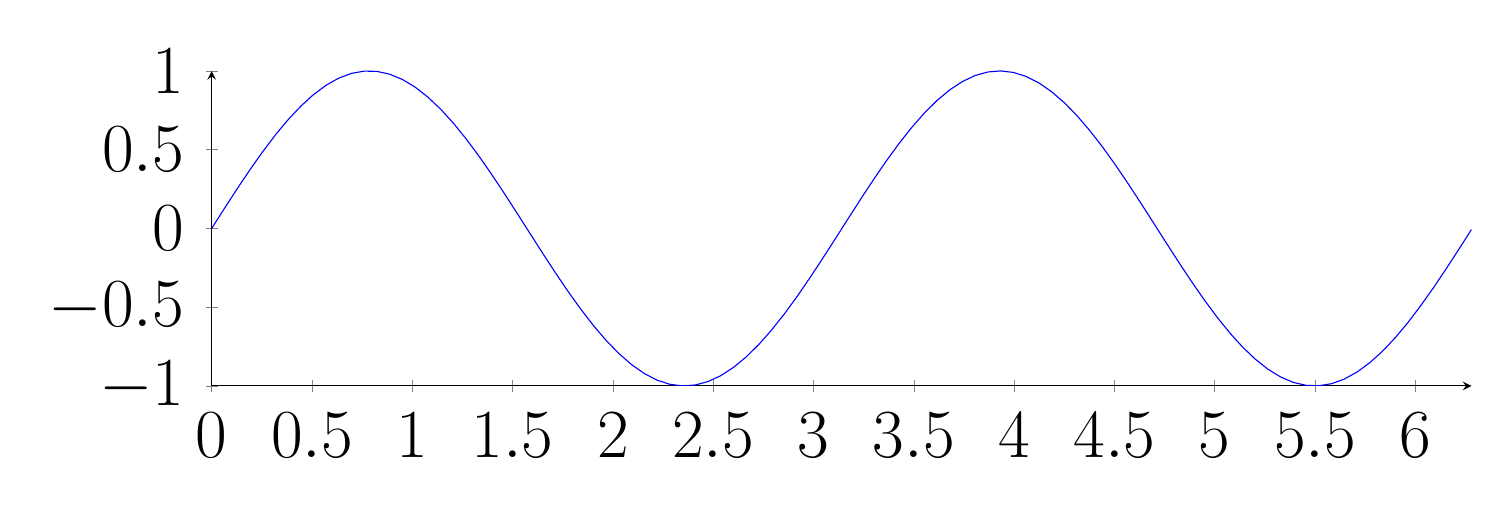
\begin{tikzpicture}
\begin{axis}[
  domain=0:6.28,
  axis lines = left,
  legend pos=outer north east,
  width=16cm,
  height=4cm,
  scale only axis,
]
\addplot [
  samples=100, 
  color=blue,
]
{sin(deg(2*x))};

\end{axis}
\end{tikzpicture}

\end{tabular}
\end{center}
\end{figure}


\medskip
\Head{Conclusion} \\
\Large \lipsum[5-5]
\end{textblock}


\end{document}
